\documentclass{article}
\usepackage[utf8]{inputenc}
\usepackage{graphicx}
\usepackage[resetfonts]{cmap}
\usepackage{lmodern}
\usepackage[czech]{babel}
\usepackage[T1]{fontenc}
\bibliographystyle{unsrt}
\usepackage[protrusion,expansion]{microtype}
\usepackage[nonewpage]{imakeidx}
\makeindex

\setlength{\parindent}{10ex}

\begin{document}
\microtypesetup{protrusion=true, expansion=true}

\setlength{\parindent}{5ex}

\section*{Úvod}
Stereoskopie\cite{wiki_stereoskopie} je dnes všeobecně známá spíše pod názvem „3D technologie“\index{3D technologie|see{Stereoskopie}}. Toto označení ale není zcela správné, 3D~=~3 dimenze (slovo dimenze\index{Dimenze}\cite{dimension} znamená rozměr - původ z~latiny). 3D\index{3D prostor} je tedy prostor, který má 3~rozměry. Takový prostor je všude kolem nás. Zatímco stereoskopie\index{Stereoskopie} je systém, který umožňuje 2D obraz (tzn. plošný, např. na papíře nebo na monitoru) vnímat jako 3D obraz. V~principu jde tedy o~zrakovou iluzi.

\section{Princip zrakového 3D vjemu}
Samotné oko vidí 2D obraz. Tím, že oko zplošťuje nebo roztahuje čočku (akomodace\index{Akomodace}), zaostřuje sice na bližší a~vzdálenější objekty v~prostoru, samotný 3D obraz ale nevytváří.\par
Podmínkou\index{3D zrakový vjem|(} 3D vnímání prostoru je mít dvě oči, jejichž osy musí směřovat stejným směrem. Tím, že jsou osy v určité vzdálenosti od sebe, každé oko vidí obraz před sebou z~jiného úhlu, a~tudíž se oba obrazy od sebe mírně liší (viz obr.~\ref{viewsDiff}). Mozek si oba obrazy automaticky spojí a~umožní nám tak vnímat třetí rozměr, tedy hloubku prostoru.\index{3D zrakový vjem|)}

\begin{figure}[htbp]
        \begin{center}
            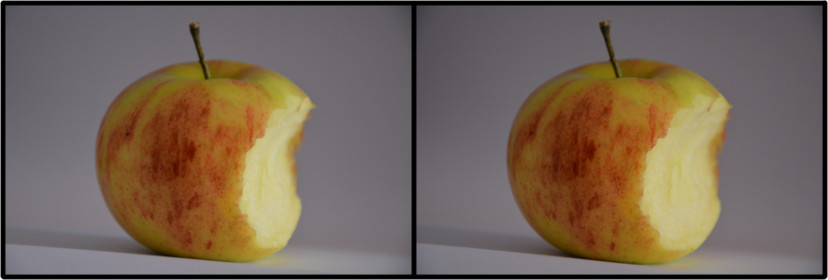
\includegraphics[width=1\textwidth]{bitmap_photo.jpg}
        \end{center}
        \caption{obraz levého oka (nalevo), obraz pravého oka (napravo)}
        \label{viewsDiff}
    \end{figure}

\subsection{Konvergence a divergence}
Čím blíže je pozorovaný objekt k~pozorovateli, tím více se oči pozorovatele přibližují k~sobě (mírně šilhají) a~zároveň se vše, co je za objektem, rozdvojuje a~vzdaluje od sebe. Tento děj se označuje jako konvergence\index{Konvergence}. Naopak, když se pozorovatel dívá na vzdálenější objekt, oči se od sebe oddalují a~dvojitě vidí bližší objekty. Tento děj se označuje jako divergence\index{Divergence}. Optické osy očí (osa určená středem sítnice a~středem čočky oka; určuje směr pozorování oka) dosáhnou maximálního oddálení tehdy, když se pozorovatel dívá „do ztracena“ (např. na obzor, na nebe). V~tomto případě budou osy rovnoběžné. Plasticky (tj. rozeznávat tvar) je člověk schopen vnímat objekty do vzdálenosti několika metrů, jednotlivé vrstvy prostoru (např. jednotlivé masivy hor) až do stovek metrů.


\vspace{5mm}
\noindent\makebox[\linewidth]{\rule{\paperwidth}{0.4pt}}

\textit{Pozn.: druhá polovina 1.~zápočtového dokumentu je část práce soč, která je mým autorským dílem. Původně byla vypracována pomocí programu Microsoft Word, pro účely tohoto dokumentu jsem ji upravil a~vysázel v~\LaTeX u.}

\bibliography{bibliography}
\printindex

\end{document}